\documentclass{article}
\usepackage{graphicx} % Required for inserting images

\title{{Krishna Dindial's Ps4}}
\author{https://github.com/kdindial/phys-ga2000 }
\date{October 2024}

\begin{document}

\maketitle

\section{Introduction}
In recitation, when you showed of your hermite(n) I liked how you made a function of n that returned a function of x.

When I started this PS, I originally wrote a a new function to evaluate the gaussian quadrature algorithm for each problem,  because each problem had its own paramaters that I wanted to vary. For example in problem 2, I made a function that evaluated the Gaussian quadrature for a given amplitude a. However, once I saw that I could output a function from another function and then pass that function into another function, I realized I only need to write one gaussian quadrature function, then I can pass any f(x) into that. When I had a problem that depended on two paramters, like an f(x,a), I could make a function f(a) that outputs an f(x). Then I just pass f(a) into my gaussian quadrature function because it takes f(a) returns f(x) and my gaussian quadrature function takes f(x) as the input.
\par
For this problem set, I included n a file called integration.py, I made a function to evaluate the gaussian polynomial quadrature, and another function to evaluate the gaus hermite quadrature. Then whenever it was time to evaluate an integral, i just imported the gausQuad function.

\section{Problem 1}
\subsection{1a}
see my github code
\subsection{1b}
In figure 1, I plot C(T) vs T
\begin{figure}[h!]
    \centering
    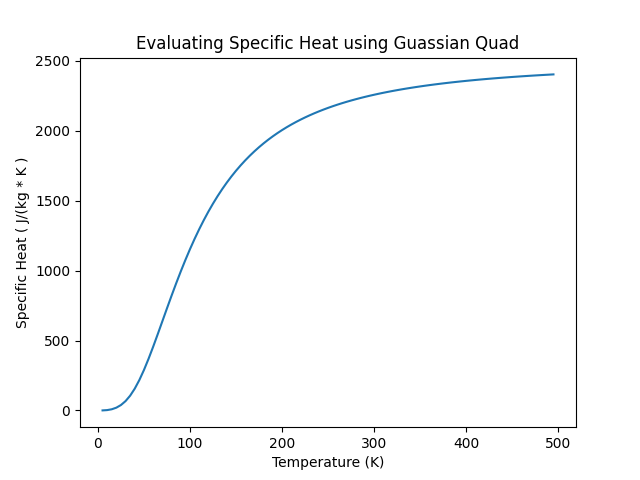
\includegraphics[width=.8\linewidth]{ps-4-1b.png}
    \caption{Specific Heat vs Temperature hsing gaussian quadrature}
    \label{fig:enter-label}
\end{figure}

\subsection{1c}
In figure 2, I  plot how the specific heat integral converges for varying Ns at T=5
\begin{figure}[h!]
    \centering
    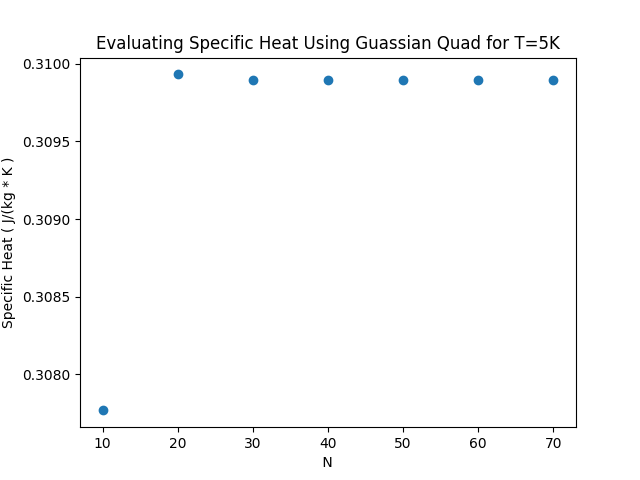
\includegraphics[width=.8\linewidth]{ps-4-1c.png}
    \caption{Gaussian Quad Converging}
    \label{fig:enter-label}
\end{figure}

\section{Problem 2}
\subsection{2a}
First we are asked to do something similar to the method of quadrature to solve for the period of an an-harmonic oscillator. We need to rearrange the equation:
\begin{equation}
    E=\frac{1}{2}m(\dot{x})^2 + V(x)
\end{equation}
into an integral that tells us the period. In dynamics class, we call this the method of quadrature. First isolate the dx/dt term:


\begin{equation}
   \sqrt{ \frac{2}{m}(E-V(x)) }=\frac{dx}{dt}
\end{equation}

Then invert everything:

\begin{equation}
   \frac{1}{\sqrt{ \frac{2}{m}(E-V(x)) }}=\frac{dt}{dx}
\end{equation}

Then "move" the dx to the other side
\begin{equation}
   \int_{x1}^{x2}\frac{dx}{\sqrt{ \frac{2}{m}(E-V(x)) }}=\int_{t1}^{t2}dt
\end{equation}

The book says: ''Let us assume that the potential V(x) is symmetric about x = 0 and let us set our anharmonic oscillator going with amplitude a. That is, at t = 0 we release it from rest at position x = a and it swings back towards the origin. Then at t = 0 we have dx I dt = 0 and the equation above reads E = V(a), which gives us the total energy of the particle in terms of the amplitude."
\par Plugging that information into equation 4: 



\begin{equation}
  \sqrt{\frac{m}{2}} \int_0^a \frac{dx}{\sqrt{ (V(a)-V(x)) }}=\int_{0}^{T/4}dt
\end{equation}

On the right side we just have T/4, so we can put it in the form that the book has by multiplying both sides by 4:

\begin{equation}
  \sqrt{8m} \int_0^a \frac{dx}{\sqrt{ (V(a)-V(x)) }}=T
\end{equation}

\section{2b}

In figure 3, you can see the period decreases as the amplitudes increases. This is because the "force" depends on -dV/dx, so the particle will feel a force of $-x^3$ in the opposite direction. The farther its displacement, it will feel a force back in the opposite direction that is $x^2$ times stronger than the simple harmonic oscillator.
\begin{figure}[h!]
    \centering
    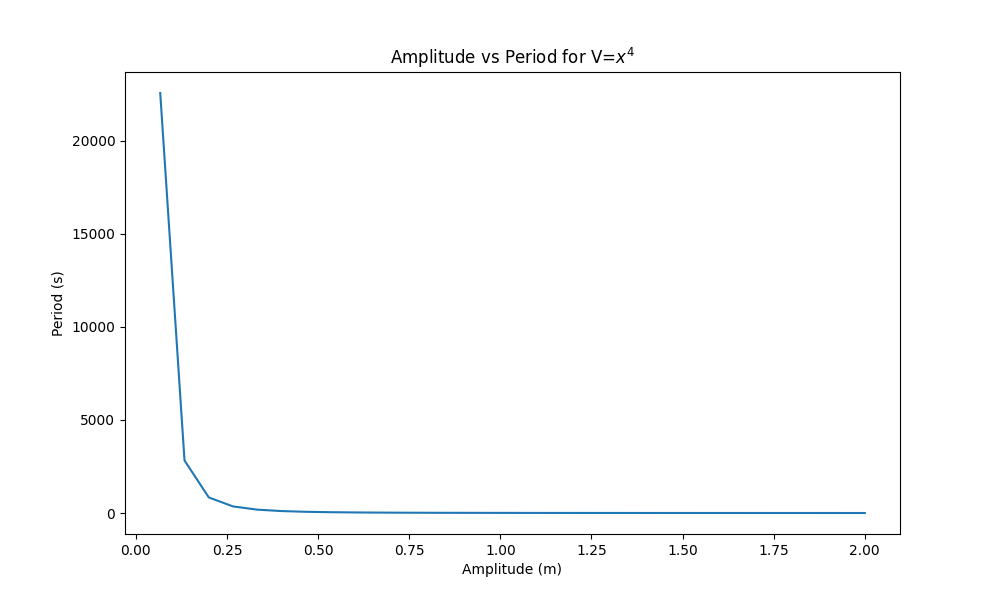
\includegraphics[width=\linewidth]{ps-4-2.png}
    \caption{Period vs amplitude}
    \label{Anharmonic Oscilator Period vs amplitude}
\end{figure}

\section{Problem 3}:
\subsection{3a}

In figure 4 you can see my plot of the wave functions of the quantum simple harmonic oscillator. x is dimensionless
\subsection{3b}
In figure 5 you can see my plot for $\psi_{30}(x)$

\subsection{3c and 3d}
\par 
For this problem I just passed in the $x^2\psi_n^2$ into the gausquad function that I used for all of the other problems. Since the integral is from -inf to inf, I remapped f(z)dz onto $\frac{f(\tan(x))dz}{\cos(x)^2}$. When I tried to evaluate this with gaus poly quadrature I got an answer that was very off. 
\par
I got that the rms was 3.3223... For a sanity check, I tried using the same procedure to calculate  $<\psi_n^2>$, which I new should just be one. My function returned 1.994665. I then tried to compare to evaluating the rms and the norm with gaus hermite quadrature and got that it was 0.1740145... Then using guas hermite quadratuer I tried to evaluate the rms and got 0.303052. This was really confusing. It makes me think my normalization of psi is wrong and my implementation of the gaussian quadrature algorithms is wrong.
\par
In figure 6 and 7 plot $x^2\psi(x)^2$ and $x^2\psi(x)^2$ to see if my functions make sense. The plots look like what I would expect, so I know that at least that part is correct. 
\par I was unable to find the error in time to figure out why my evaluations of the integrals were so off.



\begin{figure}
    \centering
    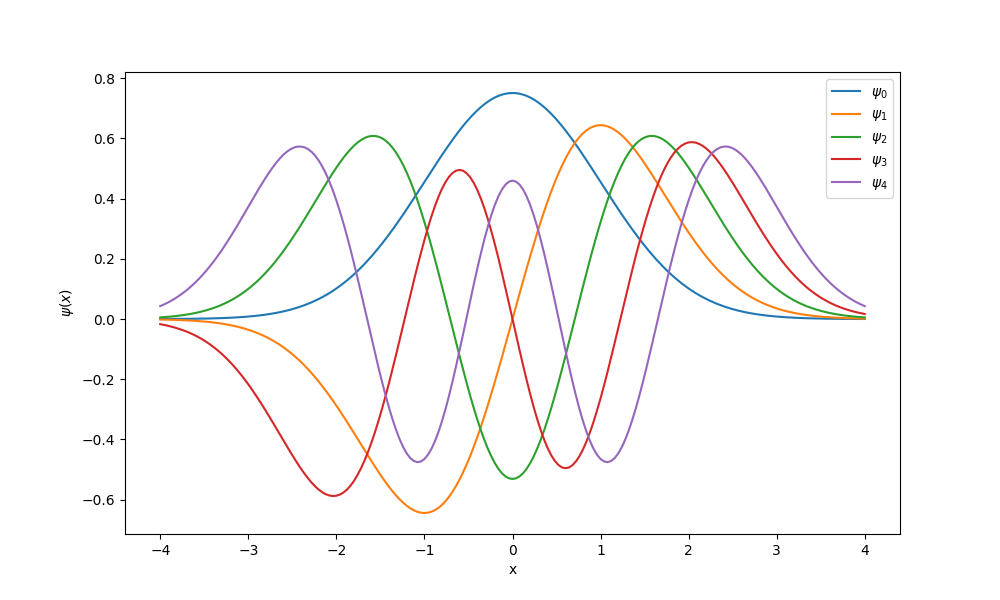
\includegraphics[width=\linewidth]{psi_1-4.png}
    \caption{sho wave function }
    \label{}
\end{figure}

\begin{figure}
    \centering
    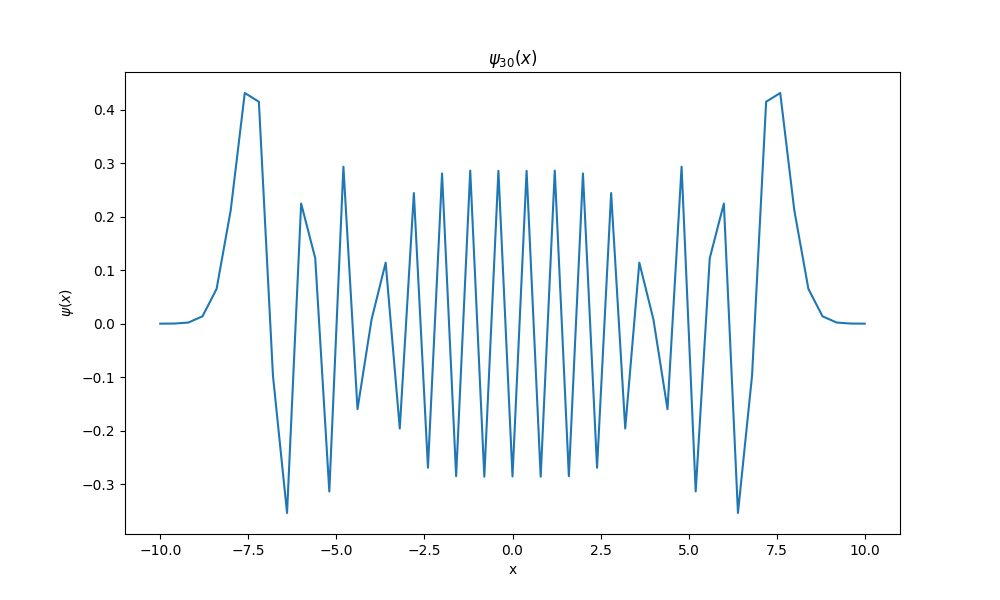
\includegraphics[width=\linewidth]{psi_30.png}
    \caption{$\psi_{30}(x)$}
    \label{fig:enter-label}
\end{figure}

\begin{figure}
    \centering
    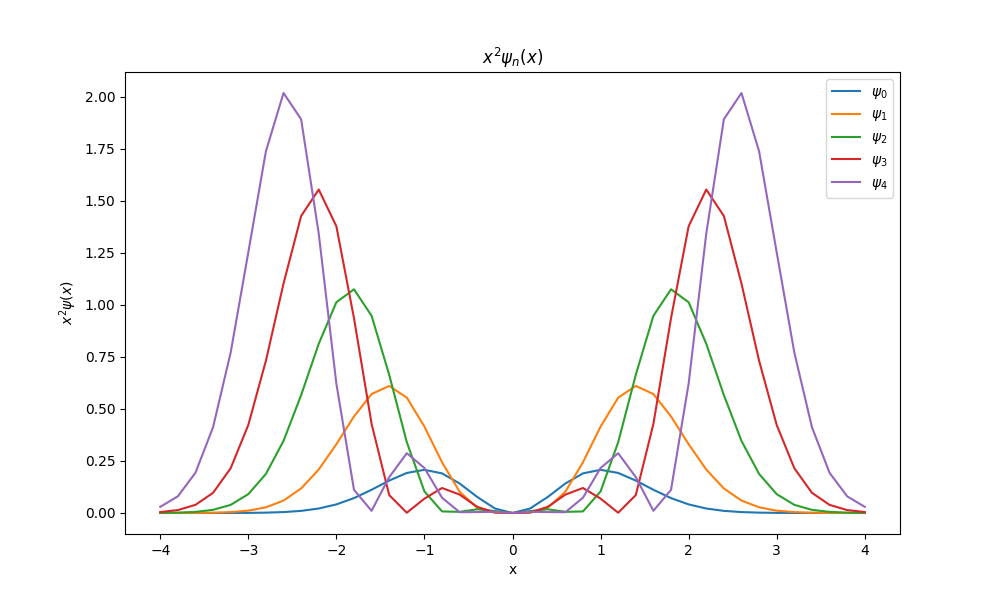
\includegraphics[width=1\linewidth]{psi_1-4_rms.png}
    \caption{$x^2\psi(x)^2$}
    \label{fig:enter-label}
\end{figure}

\begin{figure}
    \centering
    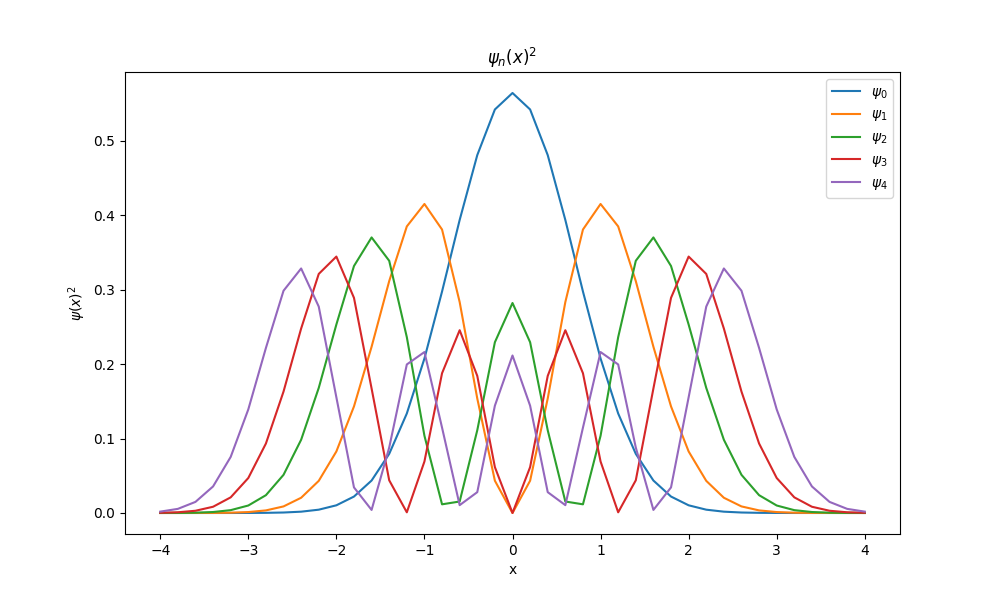
\includegraphics[width=\linewidth]{psi_1-4_norm.png}
    \caption{$x^2\psi(x)^2$}
    \label{fig:enter-label}
\end{figure}



\end{document}
